
\section{Introduction}
Precipitation plays a major role in many natural and societal systems, but direct observations of precipitation are not available for all areas. Remote sensing platforms such as satellites provide estimates of temperature via measurements of elecromagnetic radiation. Temperature and precipitation are closely related due to the physical mechanisms which govern precipitation. Furthermore there is strong spatial structure in both temperature and precipitation, so the ability to describe spatial dependence is highly desirable for models of precipitation. 

\subsection{Models}

For this project we model precipitation given temperature on a regular grid of pixels, where the values of each pixel corresponds to average amounts over a fixed time window. In order to take into account the spatial dependencies inherent in patterns of precipitation, we made conditional random fields where the precipitation values in the pixels are conditioned on temperature and other features. We tried three different methods for modeling this CRF, including Exponential Families, Logistic Regression, and Loopy BP. 

\subsection{Data Set}
We will use PERSIAN-CCS data set which consists of temperature data as well as features related to a particular cloud patch in which a pixel is part. Each pixel, which represents a small geographic area, has 1 temperature feature and 12 features related to its cloud patch. There is also a target $y$ value for that pixel obtained via radar data. The region of interest is the western United States and the temperal resolution under consideration is the finest available, 30 minutes. The following web link provides a more detailed description of the data set. 

\begin{lstlisting}
http://chrs.web.uci.edu/research/satellite_precipitation/activities01.html
\end{lstlisting}

\section{Model: Exponential Family with Conditional Random Field}

\subsection{Introduction}

Conditional Random Fields are discriminative models for the conditional distribution of labels $y$ given observations $x$. For exponential family purposes it will be defined over a graph structure as follows:
\[
p(y|x) = \frac{1}{Z(x)} \prod_i{\psi(y_i,x)} \prod_{c}{\psi(y_c,x)}
\]
Here, $Z(x)$ is the partition function that normalizes the distribution, $\psi(y_i,x)$ is the potential function for the states of node $i$ given the input $x$, and $\psi(y_c,x)$ is the potential function for the states of nodes in clique $c$ given the input $x$. The potential function are exponentials.\\
\\
We will take a 2-D image and make each pixel a separate node in our graph. Our graph will be a 4-connected grid so two pixels will be connected via an edge if they are immediate neighbors horizontally or vertically. \\
\\
Our input consists of features for each node and edge, denoted by $x_i$ and $w_c$ respectively. The edge features for clique $c$ are used to obtain a conditional distribution of values for the nodes connected by $c$ and the node features for node $i$ are used to obtain a distribution of values for only node $i$. Our equation now becomes as follows:
\[
p(y|x) = \frac{1}{Z(x)} \prod_i{\psi(y_i,x_i)} \prod_{c}{\psi(y_c,w_c)}
\]
We will learn two matrices $\theta$ and $\phi$. The matrix $\theta$ will be multiplied by the node features to determine the log potentials for each value of node $i$. The matrix $\phi$ will be multiplied by the edge features to determine the log potentials for each pair of values for the nodes $i$ and $j$ connected by an edge in our graph. The model is now as follows:
\[
p(y|x) = \frac{1}{Z(x)} \prod_i{exp(\theta x_i)} \prod_{ij}{exp(\phi w_{ij})}
\]
Our goal will be to find $\theta$ and $\phi$ matrices that minimize a loss function given our training data. Let $\mu$ be the accuracy of a clique marginal. For these results, the loss function is defined as the clique logistic loss (Domke 2013)
\[
L = - \sum_c {log \, \mu(y_c; \theta, \phi, x_i, x_j, w_c)}
\]
To perform inference on this model, Tree-Reweighted Belief Propagation was employed. This method replaces the marginal polytope with a super-set before computing the message passing updates. Approximations are done to ensure there is a tractable upper bound on the log partition function (Domke 2013). \\
\\
Truncated Fitting was employed for the learning algorithm. In summary, this method involved performing N iterations ($N=5$ for our implementation) of inference and then calculating the loss function regardless of whether or not convergence has occurred. The gradient of the loss function is then computed and this is used to update the model parameters. Finally, N iterations of inference are done in reverse order. 

\subsection{Feature Setup}

The features associated with each node are the information in the data set as well as a constant. The first node feature is temperature, thus we will define the following:
\[
\Delta x_{ij} = |x_{i1} - x_{j1}|
\]
The edge features used were inspired by computer vision labeling problems and consisted of the temperature differences between neighbors parameterized as a set of thresholds. More formally, let $T = \{ T_0 , T_1, ..., T_M \}$ be a set of thresholds. Given the set $T$ and a value $s$, we will define a function that returns a vector of which thresholds it passes as follows
\[
h(s,T) = ( \delta (s \geq T_0), \delta (s \geq T_1), ..., \delta (s \geq T_M))
\]
In our case, we will use $T_i = \frac{i}{20}$ for $i$ from $0$ to $M$ and $M=10$. For a given edge between neighbors $i$ and $j$, the edge feature vector will be as follows
\[
w_{ij} = h( \Delta x_{ij}, T)
\] 

\subsection{Results}

Our training data consisted of temperature and precipitation information from September 2011. There were readings every half hour thus there were a total of 1440 maps. Due to the large size of the data set, I used a random subset of 160 maps for training. We then tested the distribution using maps from September 2012. \\
\\
\begin{figure}[t]
\centering
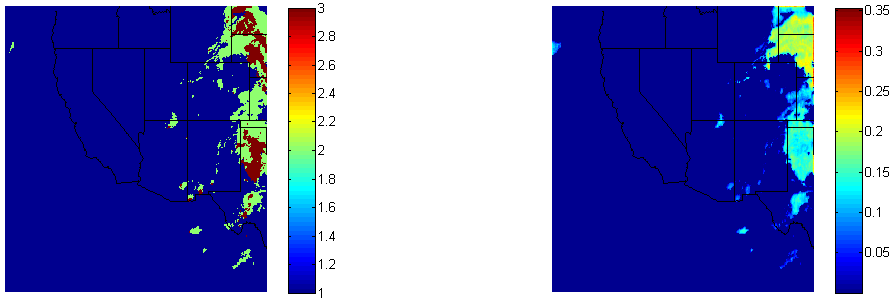
\includegraphics[height=2in]{./zackWriteUp/time698_sep2011_labelAndProb.png}
\caption{Target Labels (left) and Probability of Rainfall (right) for Sep 15, 2011 at 12:45pm. Labels mean the following: 1:No Cloud ; 2:Cloud, No Rain ; 3:Cloud, Rain}
\label{labelProb2}
\end{figure}
\begin{figure}[t]
\centering
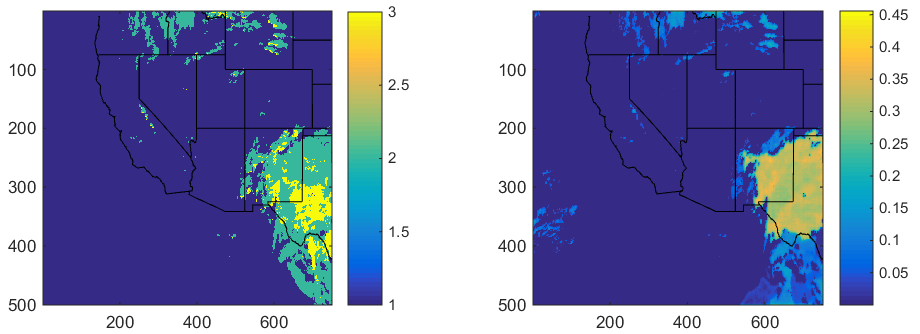
\includegraphics[height=2in]{./zackWriteUp/time1196_labelAndProb.png}
\caption{Target Labels (left) and Probability of Rainfall (right) for Dec 28, 2012 at 11:45pm. Labels mean the following: 1:No Cloud ; 2:Cloud, No Rain ; 3:Cloud, Rain}
\label{labelProb}
\end{figure}
Figure \ref{labelProb2} shows the target labels and probability of rainfall for one of the training maps. Figure \ref{labelProb} shows the same thing for one of the test maps. Results for the other maps were quite similar. The baseline error (if we predict no rain for all the cloud pixels) was $30.7\%$ for the training map and $19.9\%$ for the test map. No matter what score threshold was used for the predictor, the pixelwise error was higher than the baseline for both maps. \\
\\
The probabilities learned are at least somewhat on par with what we hoped even if they can't be used for a predictor yet. For the training map, the average marginal probability of rainfall among cloud pixels with no rain was $0.1248$ while the probability among cloud pixels with rain was $0.1547$. For the test map, the probabilities were $0.1997$ and $0.2619$ respectively.  


\subsection{Conclusion}

The results were quite discouraging so much must be needed to improve the probabilistic model. There is low probability of precipitation even in pixels where rainfall occurred. Our classes are highly imbalanced in that there are much fewer cloud pixels with rainfall than without rainfall. More needs to be done to correct for this imbalance. One problem could be that the edge features are inspired by segmentation in Computer Vision meaning that region boundaries are assumed to be quite obvious in the observed data. That has not occurred with our data thus we need to rethink what we use as our edge features in the model. The other potential problem is that our loss function sums over the clique marginals instead of calculating the likelihood over the whole map. If we attempt to optimize the likelihood over the whole map then we might obtain a better prediction. 


